
\documentclass{extbook}[14pt]
\usepackage{multicol, enumerate, enumitem, hyperref, color, soul, setspace, parskip, fancyhdr, amssymb, amsthm, amsmath, bbm, latexsym, units, mathtools}
\everymath{\displaystyle}
\usepackage[headsep=0.5cm,headheight=0cm, left=1 in,right= 1 in,top= 1 in,bottom= 1 in]{geometry}
\pagestyle{fancy}
\lhead{}
\chead{Answer Key for Final Exam: Module 1-8 Version B}
\rhead{}
\lfoot{Summer C 2020}
\cfoot{}
\rfoot{}
\begin{document}
\textbf{This key should allow you to understand why you choose the option you did (beyond just getting a question right or wrong). \href{https://xronos.clas.ufl.edu/mac1105spring2020/courseDescriptionAndMisc/Exams/LearningFromResults}{More instructions on how to use this key can be found here}.}

\textbf{If you have a suggestion to make the keys better, \href{https://forms.gle/CZkbZmPbC9XALEE88}{please fill out the short survey here}.}

\textit{Note: This key is auto-generated and may contain issues and/or errors. The keys are reviewed after each exam to ensure grading is done accurately. If there are issues (like duplicate options), they are noted in the offline gradebook. The keys are a work-in-progress to give students as many resources to improve as possible.}

\rule{\textwidth}{0.4pt}

1. Find the equation of the line described below. Write the linear equation as $ y=mx+b $ and choose the intervals that contain $m$ and $b$.
\[ \text{Parallel to } 7 x - 3 y = 3 \text{ and passing through the point } (-6, -4). \] 
The solution is $ y = 2.33x + 10.00 $ 

\begin{enumerate}[label=\Alph*.] 
\item $ m \in [-0.8, 2.2] \hspace*{3mm} b \in [8, 12] $ 

  $y = 0.43x + 10.00$, which corresponds to using the reciprocal slope $(1/m)$. 
\item $ m \in [1.1, 3.6] \hspace*{3mm} b \in [-16, -8] $ 

  $y = 2.33x - 10.00$, which corresponds to using the correct slope and getting the negative $y$-intercept. 
\item $ m \in [-2.6, -0.7] \hspace*{3mm} b \in [-23, -17] $ 

  $y = -2.33x - 18.00$, which corresponds to using the negative slope. 
\item $ m \in [1.1, 3.6] \hspace*{3mm} b \in [-1, 7] $ 

  $y = 2.33x + 2.00$, which corresponds to correct slope and mis-distributing while simplifying to slope-intercept form. 
\item $ m \in [1.1, 3.6] \hspace*{3mm} b \in [8, 12] $ 

 * $y = 2.33x + 10.00$, which is the correct option. 
\end{enumerate} 
 
\textbf{General Comment:} Parallel slope is the same and perpendicular slope is opposite reciprocal. Opposite reciprocal means flipping the fraction and changing the sign (positive to negative or negative to positive). 

-----------------------------------------------

2. Which of the following intervals describes the Range of the function below?
\[ f(x) = -\log_2{(x+5)}+5 \] 
The solution is $ (\infty, \infty) $ 

\begin{enumerate}[label=\Alph*.] 
\item $ (-\infty, a), a \in [-9, -4] $ 

 $(-\infty, -5)$, which corresponds to using the using the negative of vertical shift on $(0, \infty)$. 
\item $ [a, \infty), a \in [-1, 10] $ 

 $[5, \infty)$, which corresponds to using the negative of the horizontal shift AND including the endpoint. 
\item $ [a, \infty), a \in [-9, -4] $ 

 $[5, \infty)$, which corresponds to using the flipped Domain AND including the endpoint. 
\item $ (-\infty, a), a \in [-1, 10] $ 

 $(-\infty, 5)$, which corresponds to using the vertical shift while the Range is $(-\infty, \infty)$. 
\item $ (-\infty, \infty) $ 

 *This is the correct option. 
\end{enumerate} 
 
\textbf{General Comment:} \textbf{General Comments}: The domain of a basic logarithmic function is $(0, \infty)$ and the Range is $(-\infty, \infty)$. We can use shifts when finding the Domain, but the Range will always be all Real numbers. 

-----------------------------------------------

3. Write the equation of the graph presented below in the form $f(x)=ax^2+bx+c$, assuming  $a=1$ or $a=-1$. Then, choose the intervals that $a, b,$ and $c$ belong to.
\begin{center} 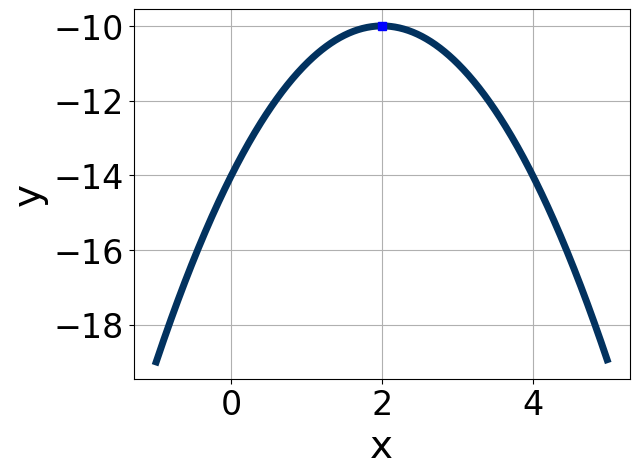
\includegraphics[width=0.3\textwidth]{../Figures/quadraticGraphToEquationB.png} \end{center} 

The solution is $ f(x) = x^{2} +4 x -6 $ 

\begin{enumerate}[label=\Alph*.] 
\item $ a \in [-5, 0], \hspace*{5mm} b \in [3, 5], \text{ and } \hspace*{5mm} c \in [-18, -13] $ 

 $f(x)=-x^{2} +4 x -14$, which corresponds to incorrectly using vertex form as $f(x) = a(x+h)^2+k$ AND making $a$ the opposite sign than it should be. 
\item $ a \in [-5, 0], \hspace*{5mm} b \in [-8, -2], \text{ and } \hspace*{5mm} c \in [-18, -13] $ 

 $f(x)=-x^{2} -4 x -14$, which corresponds to making $a$ the opposite sign than it should be. 
\item $ a \in [0, 2], \hspace*{5mm} b \in [3, 5], \text{ and } \hspace*{5mm} c \in [-8, -5] $ 

 * $f(x)=x^{2} +4 x -6$, which is the correct option. 
\item $ a \in [0, 2], \hspace*{5mm} b \in [-8, -2], \text{ and } \hspace*{5mm} c \in [13, 17] $ 

 $f(x)=x^{2} -4 x + 14$, which corresponds to incorrectly using vertex form as $f(x) = a(x+h)^2 - k$. 
\item $ a \in [0, 2], \hspace*{5mm} b \in [-8, -2], \text{ and } \hspace*{5mm} c \in [-8, -5] $ 

 $f(x)=x^{2} -4 x -6$, which corresponds to incorrectly using vertex form as $f(x) = a(x+h)^2+k$. 
\end{enumerate} 
 
\textbf{General Comment:} General Comments: When the graph is pointing up, $a=1$. When the graph is pointing down, $a=-1$. Be sure to use Vertex Form: $y = a(x-h)^2+k$. 

-----------------------------------------------

4. Construct the lowest-degree polynomial given the zeros below. Then, choose the intervals that contain the coefficients of the polynomial in the form $ax^3+bx^2+cx+d$.
\[ \frac{2}{5}, \frac{-3}{2}, \text{ and } -6 \] 
The solution is $ 10x^{3} +71 x^{2} +60 x -36 $ 

\begin{enumerate}[label=\Alph*.] 
\item $ a \in [2, 15], b \in [67, 74], c \in [57, 62], \text{ and } d \in [-40, -33] $ 

 * $10x^{3} +71 x^{2} +60 x -36$, which is the correct option. 
\item $ a \in [2, 15], b \in [43, 51], c \in [-73, -62], \text{ and } d \in [-40, -33] $ 

 $10x^{3} +49 x^{2} -72 x -36$, which corresponds to multiplying out $(5x + 5)(2x + 2)(x -1)$. 
\item $ a \in [2, 15], b \in [67, 74], c \in [57, 62], \text{ and } d \in [34, 42] $ 

 $10x^{3} +71 x^{2} +60 x + 36$, which corresponds to multiplying everything correctly except the constant term. 
\item $ a \in [2, 15], b \in [78, 84], c \in [114, 121], \text{ and } d \in [34, 42] $ 

 $10x^{3} +79 x^{2} +120 x + 36$, which corresponds to multiplying out $(5x + 5)(2x -2)(x -1)$. 
\item $ a \in [2, 15], b \in [-74, -65], c \in [57, 62], \text{ and } d \in [34, 42] $ 

 $10x^{3} -71 x^{2} +60 x + 36$, which corresponds to multiplying out $(5x + 2)(2x -3)(x -6)$. 
\end{enumerate} 
 
\textbf{General Comment:} General Comments: To construct the lowest-degree polynomial, you want to multiply out $(5x -2)(2x + 3)(x + 6)$ 

-----------------------------------------------

0. Solve the linear inequality below. Then, choose the constant and interval combination that describes the solution set.
\[ -8x -10 < 10x + 9 \] 
The solution is $ (-1.056, \infty) $ 

\begin{enumerate}[label=\Alph*.] 
\item $ (-\infty, a), \text{ where } a \in [-1, 3] $ 

  $(-\infty, 1.056)$, which corresponds to switching the direction of the interval AND negating the endpoint. You likely did this if you did not flip the inequality when dividing by a negative as well as not moving values over to a side properly. 
\item $ (a, \infty), \text{ where } a \in [-2.2, -0.7] $ 

 * $(-1.056, \infty)$, which is the correct option. 
\item $ (-\infty, a), \text{ where } a \in [-4, 1] $ 

  $(-\infty, -1.056)$, which corresponds to switching the direction of the interval. You likely did this if you did not flip the inequality when dividing by a negative! 
\item $ (a, \infty), \text{ where } a \in [0.5, 2.2] $ 

  $(1.056, \infty)$, which corresponds to negating the endpoint of the solution. 
\item $ \text{None of the above}. $ 

 You may have chosen this if you thought the inequality did not match the ends of the intervals. 
\end{enumerate} 
 
\textbf{General Comment:} General Comments: Remember that less/greater than or equal to includes the endpoint, while less/greater do not. Also, remember that you need to flip the inequality when you multiply or divide by a negative. 

-----------------------------------------------

1. Which of the following equations \textit{could} be of the graph presented below?
\begin{center} 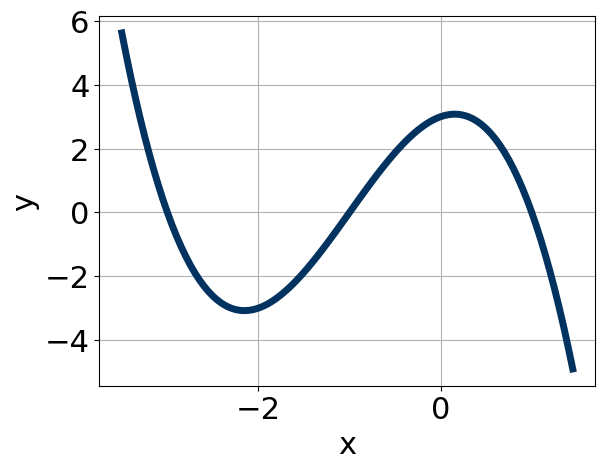
\includegraphics[width=0.3\textwidth]{../Figures/polyGraphToFunctionB.png} \end{center} 

The solution is $ 12(x - 3)^{10} (x + 4)^{6} (x - 2)^{5} $ 

\begin{enumerate}[label=\Alph*.] 
\item $ 15(x - 3)^{10} (x + 4)^{5} (x - 2)^{8} $ 

 The factor $(x + 4)$ should have an even power and the factor $(x - 2)$ should have an odd power. 
\item $ -18(x - 3)^{8} (x + 4)^{8} (x - 2)^{7} $ 

 This corresponds to the leading coefficient being the opposite value than it should be. 
\item $ -11(x - 3)^{6} (x + 4)^{6} (x - 2)^{4} $ 

 The factor $(x - 2)$ should have an odd power and the leading coefficient should be the opposite sign. 
\item $ 12(x - 3)^{10} (x + 4)^{6} (x - 2)^{5} $ 

 * This is the correct option. 
\item $ 14(x - 3)^{6} (x + 4)^{9} (x - 2)^{9} $ 

 The factor $(x + 4)$ should have an even power. 
\end{enumerate} 
 
\textbf{General Comment:} General Comments: Draw the x-axis to determine which zeros are touching (and so have even multiplicity) or cross (and have odd multiplicity). 

-----------------------------------------------

2. What is the domain of the function below?
\[ f(x) = \sqrt[8]{7 x + 8} \] 
The solution is $ [-1.143, \infty) $ 

\begin{enumerate}[label=\Alph*.] 
\item $ [a, \infty), \text{ where } a \in [-1.69, -1.01] $ 

 * $[-1.143, \infty)$, which is the correct option. 
\item $ (-\infty, \infty) $ 

 This corresponds to the radical having an odd power, but the radical for this question is even. 
\item $ (-\infty, a], \text{where } a \in [-0.94, -0.45] $ 

 $(-\infty, -0.875]$, which corresponds to reversing the direction of the domain AND using the negative of the correct pivot value. 
\item $ [a, \infty), \text{where } a \in [-1.12, 0.23] $ 

 $[-0.875, \infty)$, which corresponds to using the negative of the correct pivot value. 
\item $ (-\infty, a], \text{where } a \in [-2.4, -1.08] $ 

  $(-\infty, -1.143]$, which corresponds to reversing the direction of the domain. 
\end{enumerate} 
 
\textbf{General Comment:} Remember that we cannot take the even root of a negative number - this is why the domain is only sometimes restricted! If we have an even root, we solve $7 x + 8 \geq 0$. Since this is an inequality, remember to flip the inequality if we divide by a negative number. 

-----------------------------------------------

3. Solve the linear equation below. Then, choose the interval that contains the solution.
\[ \frac{-5x + 7}{2} - \frac{-7x -9}{3} = \frac{8x + 4}{7} \] 
The solution is $ x = 4.527 $ 

\begin{enumerate}[label=\Alph*.] 
\item $ x \in [3.6, 5.4] $ 

 * $x = 4.527$, which is the correct option. 
\item $ x \in [0.8, 1.4] $ 

  $x = 0.988$, which corresponds to dividing the second number in the numerator by the denominator rather than dividing BOTH parts of the numerator by the denominator (or removing the fractions through multiplication). 
\item $ x \in [8.9, 10] $ 

  $x = 9.164$, which corresponds to dividing the coefficients in front of x by the denominator rather than dividing BOTH parts of the numerator by the denominator (or removing the fractions through multiplication). 
\item $ x \in [-0.8, 0.8] $ 

  $x = -0.055$, which corresponds to not distributing the negative in front of the second fraction. 
\item $ \text{There are no real solutions.} $ 

 Corresponds to students thinking a fraction means there is no solution to the equation. 
\end{enumerate} 
 
\textbf{General Comment:} If you are having trouble with this problem, try to remove a fraction at a time by multiplying each term by the denominator. 

-----------------------------------------------

4. First, find the equation of the line containing the two points below. Then, write the equation as $ y=mx+b $ and choose the intervals that contain $m$ and $b$.
\[ (-3, 5) \text{ and } (8, -8) \] 
The solution is $ y = -1.18x + 1.45 $ 

\begin{enumerate}[label=\Alph*.] 
\item $ m \in [-7, 0] \hspace*{3mm} b \in [1.44, 2.15] $ 

 * $y = -1.18x + 1.45$, which is the correct option. 
\item $ m \in [-7, 0] \hspace*{3mm} b \in [7.72, 8.05] $ 

  $y = -1.18x + 8.0$, which corresponds to using the correct slope/equation but not distributing correctly using the first point. 
\item $ m \in [0, 3] \hspace*{3mm} b \in [-17.89, -16.45] $ 

  $y = 1.18x -17.45$, which corresponds to using the negative slope and the correct equation. 
\item $ m \in [-7, 0] \hspace*{3mm} b \in [-1.59, -0.27] $ 

  $y = -1.18x -1.45$, which corresponds to using the correct slope and getting the negative y-intercept. 
\item $ m \in [-7, 0] \hspace*{3mm} b \in [-16.36, -15.83] $ 

  $y = -1.18x -16.0$, which corresponds to using the correct slope/equation but not distributing correctly using the second point. 
\end{enumerate} 
 
\textbf{General Comment:} Remember to keep your points in order when plugging in to the slope formula. 

-----------------------------------------------

0. Solve the linear inequality below. Then, choose the constant and interval combination that describes the solution set.
\[ -9 - 9 x \leq \frac{-13 x - 9}{5} < 4 - 3 x \] 
The solution is $ \text{None of the above.} $ 

\begin{enumerate}[label=\Alph*.] 
\item $ (-\infty, a) \cup [b, \infty), \text{ where } a \in [-0.5, 1.4] \text{ and } b \in [-18, -10] $ 

 $(-\infty, 1.12) \cup [-14.50, \infty)$, which corresponds to displaying the and-inequality as an or-inequality AND flipping the inequality AND getting negatives of the actual endpoints. 
\item $ [a, b), \text{ where } a \in [0.7, 1.3] \text{ and } b \in [-15, -13] $ 

 $[1.12, -14.50)$, which is the correct interval but negatives of the actual endpoints. 
\item $ (a, b], \text{ where } a \in [-1, 2] \text{ and } b \in [-16, -13] $ 

 $(1.12, -14.50]$, which corresponds to flipping the inequality and getting negatives of the actual endpoints. 
\item $ (-\infty, a] \cup (b, \infty), \text{ where } a \in [0, 2] \text{ and } b \in [-15, -12] $ 

 $(-\infty, 1.12] \cup (-14.50, \infty)$, which corresponds to displaying the and-inequality as an or-inequality and getting negatives of the actual endpoints. 
\item $ \text{None of the above.} $ 

 * This is correct as the answer should be $[-1.12, 14.50)$. 
\end{enumerate} 
 
\textbf{General Comment:} To solve, you will need to break up the compound inequality into two inequalities. Be sure to keep track of the inequality! It may be best to draw a number line and graph your solution. 

-----------------------------------------------

1. Graph the equation below.
\[ f(x) = (x+1)^2 + 12 \] 

 
 The solution is  
 \begin{center} 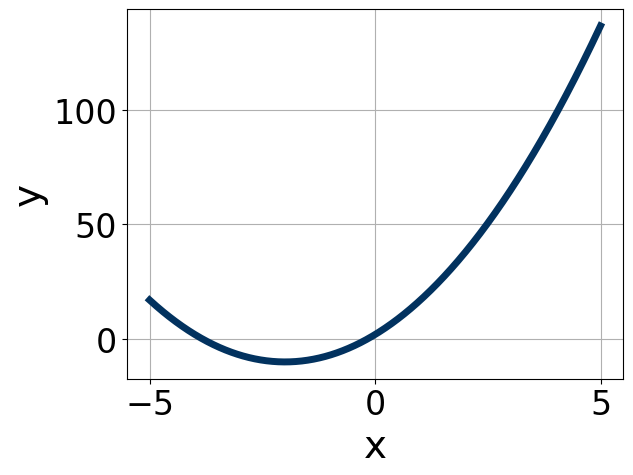
\includegraphics[width=0.3\textwidth]{../Figures/quadraticEquationToGraphBB.png} \end{center}\begin{tabular}{|c|c|} 
\hline 
 & \tabularnewline 
 \textbf{A.} 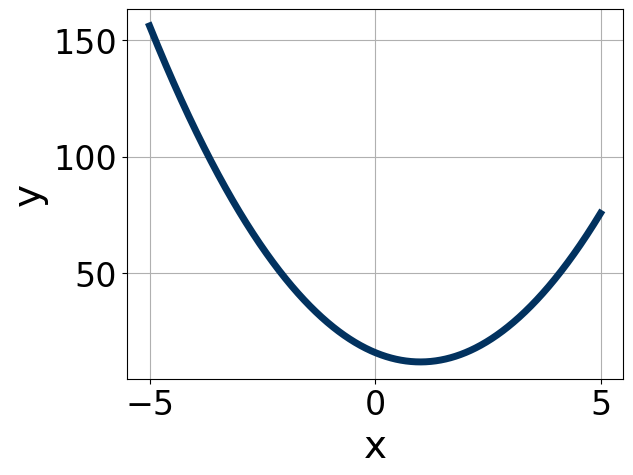
\includegraphics[width=0.3\textwidth]{../Figures/quadraticEquationToGraphAB.png} & \textbf{B.} 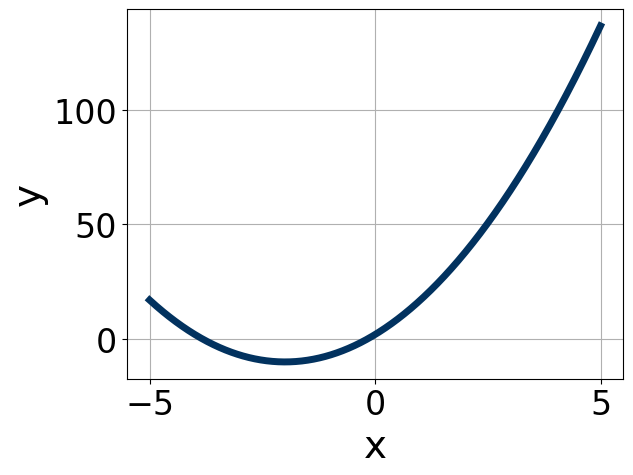
\includegraphics[width=0.3\textwidth]{../Figures/quadraticEquationToGraphBB.png} \tabularnewline 
\hline 
 & \tabularnewline 
 \textbf{C.} 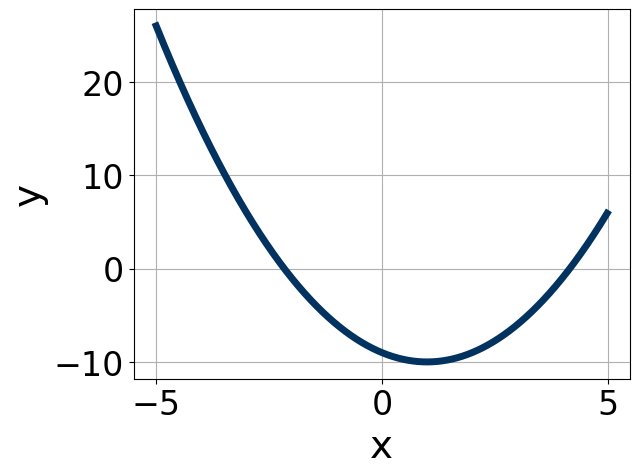
\includegraphics[width=0.3\textwidth]{../Figures/quadraticEquationToGraphCB.png} & \textbf{D.} 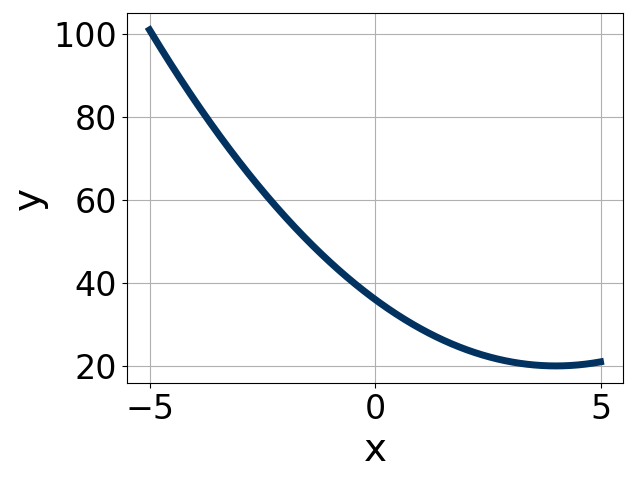
\includegraphics[width=0.3\textwidth]{../Figures/quadraticEquationToGraphDB.png} \tabularnewline 
\hline 
 E. None of the figures above. & \tabularnewline 
\hline 
 \end{tabular} 
 
\begin{enumerate}[label=\Alph*.] 
\item Used the incorrect general form $f(x) = a(x+h)^2 + k$  
\item This is the correct option.  
\item Used the incorrect general form $f(x) = -a(x-h)^2 + k$  
\item Used the incorrect general form $f(x) = -a(x+h)^2 + k$  
\end{enumerate} 
 
\textbf{General Comment:} General Comments: Remember that Vertex Form is $y = a(x-h)^2+k$, where the vertex is $(h, k)$. 

-----------------------------------------------

2. Solve the quadratic equation below. Then, choose the intervals that the solutions belong to, with $x_1 \leq x_2$ (if they exist).
\[ 10x^{2} +14 x -2 = 0 \] 
The solution is $ x_1 = -1.531 \text{ and } x_2 = 0.131 $ 

\begin{enumerate}[label=\Alph*.] 
\item $ x_1 \in [-16.2, -14.9] \text{ and } x_2 \in [1.26, 1.34] $ 

  $x_1 = -15.307 \text{ and } x_2 = 1.307$, which corresponds to using the Quadratic Formula with $a=1$ 
\item $ x_1 \in [-1.2, 1.4] \text{ and } x_2 \in [1.36, 2.66] $ 

  $x_1 = -0.131 \text{ and } x_2 = 1.531$, which corresponds to writing the Quadratic Formula as $\frac{b \pm \sqrt{b^2 - 4ac}}{2a}$ 
\item $ x_1 \in [-18, -16.9] \text{ and } x_2 \in [15.75, 16.04] $ 

  $x_1 = -17.313 \text{ and } x_2 = 15.913$, which corresponds to writing the Quadratic Formula as $-\frac{b}{2a} \pm \sqrt{b^2 - 4ac}$. 
\item $ x_1 \in [-1.7, -1.3] \text{ and } x_2 \in [-0.25, 0.43] $ 

 * $x_1 = -1.531 \text{ and } x_2 = 0.131$, which is the correct option. 
\item $ \text{There are no Real solutions.} $ 

 Corresponds to getting a negative under the radical or believing that since the quadratic cannot be factored, it has no Real solutions. 
\end{enumerate} 
 
\textbf{General Comment:} General Comments: This requires Quadratic Formula. Just be sure to use the correct formula and watch your signs. 

-----------------------------------------------

3. Choose the graph of the equation below.
\[ f(x) = - \sqrt[3]{x + 12} + 4 \] 

 
 The solution is  
 \begin{center} 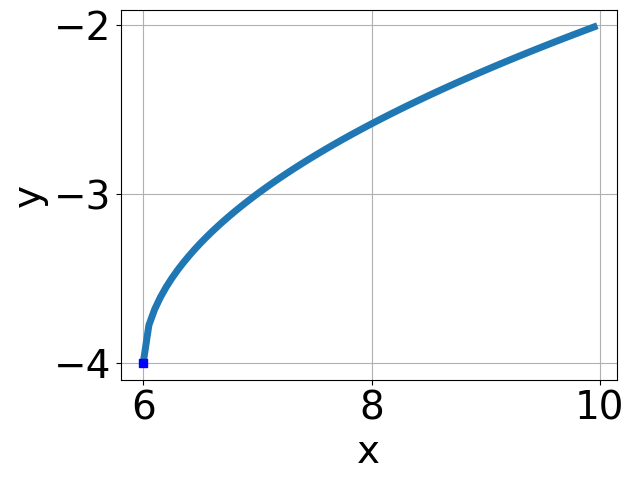
\includegraphics[width=0.3\textwidth]{../Figures/radicalEquationToGraphDB.png} \end{center}\begin{tabular}{|c|c|} 
\hline 
 & \tabularnewline 
 \textbf{A.} 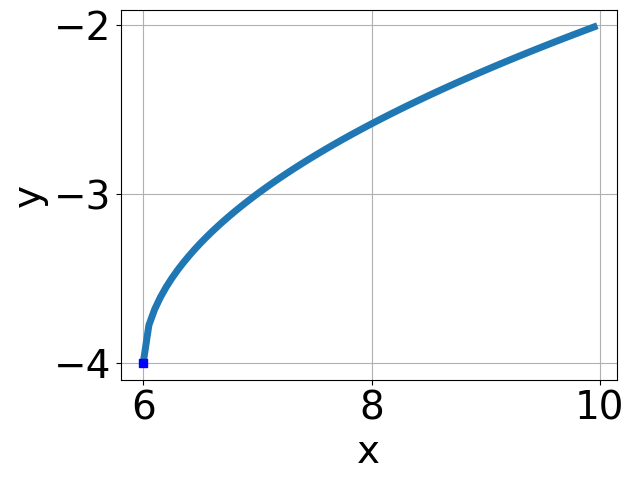
\includegraphics[width=0.3\textwidth]{../Figures/radicalEquationToGraphDB.png} & \textbf{B.} 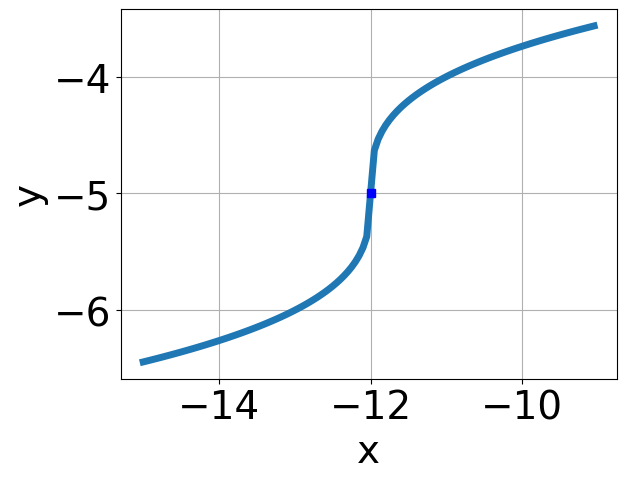
\includegraphics[width=0.3\textwidth]{../Figures/radicalEquationToGraphBB.png} \tabularnewline 
\hline 
 & \tabularnewline 
 \textbf{C.} 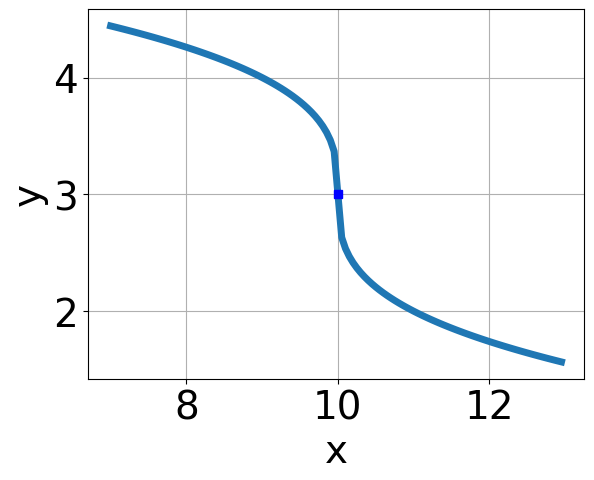
\includegraphics[width=0.3\textwidth]{../Figures/radicalEquationToGraphAB.png} & \textbf{D.} 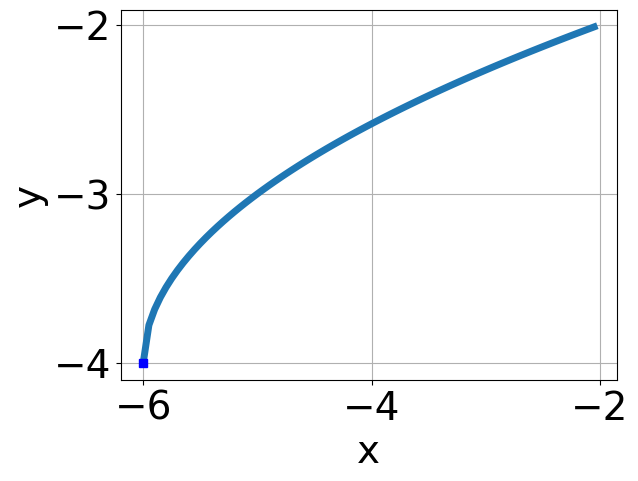
\includegraphics[width=0.3\textwidth]{../Figures/radicalEquationToGraphCB.png} \tabularnewline 
\hline 
 E. None of the figures above. & \tabularnewline 
\hline 
 \end{tabular} 
 
\begin{enumerate}[label=\Alph*.] 
\item * This is the correct option.  
\item Corresponds to switching the coefficient and having the correct vertex.  
\item Corresponds to the correct coefficient and switching the $x$-value of the vertex.  
\item Corresponds to switching the coefficient AND switching the $x$-value of the vertex.  
\end{enumerate} 
 
\textbf{General Comment:} General Comments: Remember that the general form of a radical equation is $ f(x) = a \sqrt[b]{x - h} + k $, where $a$ is the leading coefficient (and in this case, we assume is either 1 or -1), $b$ is the root degree (in this case, either 2 or 3), and $(h, k)$ is the vertex. 

-----------------------------------------------

4. Which of the following intervals describes the Range of the function below?
\[ f(x) = -e^{x+8}-3 \] 
The solution is $ (-\infty, -3) $ 

\begin{enumerate}[label=\Alph*.] 
\item $ [a, \infty), a \in [1, 7] $ 

 $[3, \infty)$, which corresponds to using the negative vertical shift AND flipping the Range interval AND including the endpoint. 
\item $ (a, \infty), a \in [1, 7] $ 

 $(3, \infty)$, which corresponds to using the negative vertical shift AND flipping the Range interval. 
\item $ (-\infty, a), a \in [-11, 2] $ 

 * $(-\infty, -3)$, which is the correct option. 
\item $ (-\infty, a], a \in [-11, 2] $ 

 $(-\infty, -3]$, which corresponds to including the endpoint. 
\item $ (-\infty, \infty) $ 

 This corresponds to confusing range of an exponential function with the domain of an exponential function. 
\end{enumerate} 
 
\textbf{General Comment:} \textbf{General Comments}: Domain of a basic exponential function is $(-\infty, \infty)$ while the Range is $(0, \infty)$. We can shift these intervals [and even flip when $a<0$!] to find the new Domain/Range. 

-----------------------------------------------

0. Solve the rational equation below. Then, choose the interval(s) that the solution(s) belongs to.
\[ \frac{2x}{7x + 7} + \frac{-4x^{2}}{-42x^{2} + 42} = \frac{-6}{-6x + 6} \] 
The solution is $ \text{There are two solutions: } x = -0.652 \text{ and } x = 4.027 $ 

\begin{enumerate}[label=\Alph*.] 
\item $ x_1 \in [-2.16, 0.41] \text{ and } x_2 \in [-3,1] $ 

  
\item $ \text{All solutions lead to invalid or complex values in the equation.} $ 

  
\item $ x_1 \in [-2.16, 0.41] \text{ and } x_2 \in [0,5] $ 

 * $x = -0.652 \text{ and } x = 4.027$, which is the correct option. 
\item $ x \in [0.82,1.3] $ 

  
\item $ x \in [3,4.15] $ 

  
\end{enumerate} 
 
\textbf{General Comment:} General Comments: Distractors are different based on the number of solutions. Remember that after solving, we need to make sure our solution does not make the original equation divide by zero! 

-----------------------------------------------

1. Describe the zero behavior of the zero $x = -6$ of the polynomial below.
\[ f(x) = 5(x + 7)^{6}(x - 7)^{5}(x - 6)^{10}(x + 6)^{5} \] 

 
 The solution is  
 \begin{center} 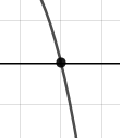
\includegraphics[width=0.3\textwidth]{../Figures/polyZeroBehaviorAB.png} \end{center}\begin{tabular}{|c|c|} 
\hline 
 & \tabularnewline 
 \textbf{A.} 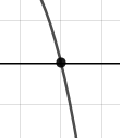
\includegraphics[width=0.3\textwidth]{../Figures/polyZeroBehaviorAB.png} & \textbf{B.} 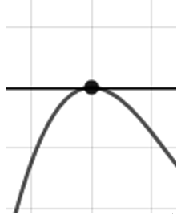
\includegraphics[width=0.3\textwidth]{../Figures/polyZeroBehaviorBB.png} \tabularnewline 
\hline 
 & \tabularnewline 
 \textbf{C.} 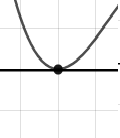
\includegraphics[width=0.3\textwidth]{../Figures/polyZeroBehaviorCB.png} & \textbf{D.} 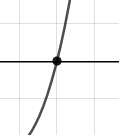
\includegraphics[width=0.3\textwidth]{../Figures/polyZeroBehaviorDB.png} \tabularnewline 
\hline 
 E. None of the figures above. & \tabularnewline 
\hline 
 \end{tabular} 
 
\begin{enumerate}[label=\Alph*.] 
\item   
\item   
\item   
\item   
\end{enumerate} 
 
\textbf{General Comment:} \textbf{General Comments:} You will need to sketch the entire graph, then zoom in on the zero the question asks about. 

-----------------------------------------------

2. Choose the equation of the function graphed below.
\begin{center} 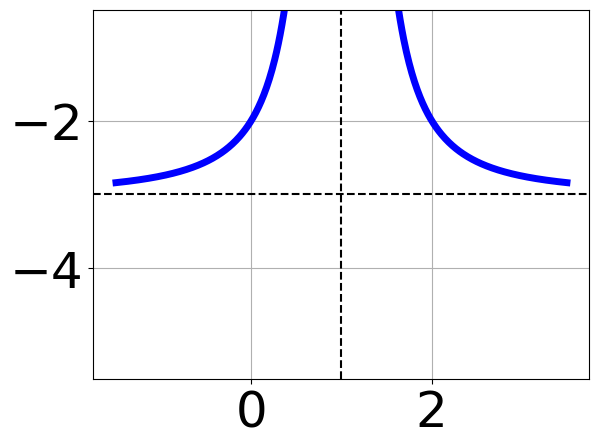
\includegraphics[width=0.3\textwidth]{../Figures/rationalGraphToEquationB.png} \end{center} 

The solution is $ \text{None of the above as it should be } f(x) = \frac{1}{x + 3} - 2 $ 

\begin{enumerate}[label=\Alph*.] 
\item $ f(x) = \frac{-1}{x - 3} - 8 $ 

 Corresponds to using the general form $f(x) = \frac{a}{x+h}+k$, the opposite leading coefficient AND not noticing the $y$-value was wrong. 
\item $ f(x) = \frac{-1}{(x - 3)^2} - 8 $ 

 Corresponds to thinking the graph was a shifted version of $\frac{1}{x^2}$, using the general form $f(x) = \frac{a}{x+h}+k$, the opposite leading coefficient, AND not noticing the $y$-value was wrong. 
\item $ f(x) = \frac{1}{x + 3} - 8 $ 

 The $y$-value of the equation does not match the graph. 
\item $ f(x) = \frac{1}{(x + 3)^2} - 8 $ 

 Corresponds to thinking the graph was a shifted version of $\frac{1}{x^2}$ not noticing the $y$-value was wrong. 
\item $ \text{None of the above} $ 

 None of the equation options were the correct equation. 
\end{enumerate} 
 
\textbf{General Comment:} General Comments: Remember that the general form of a basic rational equation is $ f(x) = \frac{a}{(x-h)^n} + k$, where $a$ is the leading coefficient (and in this case, we assume is either $1$ or $-1$), $n$ is the degree (in this case, either $1$ or $2$), and $(h, k)$ is the intersection of the asymptotes. 

-----------------------------------------------

3. Solve the linear equation below. Then, choose the interval that contains the solution.
\[ \frac{-4x -3}{8} - \frac{-3x -9}{4} = \frac{9x -8}{7} \] 
The solution is $ x = 2.914 $ 

\begin{enumerate}[label=\Alph*.] 
\item $ x \in [2.7, 4.1] $ 

 * $x = 2.914$, which is the correct option. 
\item $ x \in [-1.7, -0.3] $ 

  $x = -1.431$, which corresponds to not distributing the negative in front of the second fraction. 
\item $ x \in [12.8, 14.2] $ 

  $x = 13.517$, which corresponds to dividing the coefficients in front of x by the denominator rather than dividing BOTH parts of the numerator by the denominator (or removing the fractions through multiplication). 
\item $ x \in [-0.1, 0.8] $ 

  $x = 0.302$, which corresponds to dividing the second number in the numerator by the denominator rather than dividing BOTH parts of the numerator by the denominator (or removing the fractions through multiplication). 
\item $ \text{There are no real solutions.} $ 

 Corresponds to students thinking a fraction means there is no solution to the equation. 
\end{enumerate} 
 
\textbf{General Comment:} If you are having trouble with this problem, try to remove a fraction at a time by multiplying each term by the denominator. 

-----------------------------------------------

4. Solve the equation for $x$ and choose the interval that contains the solution (if it exists).
\[ 4^{-4x-2} = 49^{-3x+2} \] 
The solution is $ x = 1.722 $ 

\begin{enumerate}[label=\Alph*.] 
\item $ x \in [-0.1, 0.7] $ 

 $x = 0.652$, which corresponds to distributing the $\ln(base)$ to the first term of the exponent only. 
\item $ x \in [-11.9, -10.2] $ 

 $x = -10.556$, which corresponds to distributing the $\ln(base)$ to the second term of the exponent only. 
\item $ x \in [0.8, 2.5] $ 

 * $x = 1.722$, which is the correct option. 
\item $ x \in [-5, -2.1] $ 

 $x = -4.000$, which corresponds to solving the numerators as equal while ignoring the bases are different. 
\item $ \text{There is no Real solution to the equation.} $ 

 This corresponds to believing there is no solution since the bases are not powers of each other. 
\end{enumerate} 
 
\textbf{General Comment:} \textbf{General Comments:} This question was written so that the bases could not be written the same. You will need to take the log of both sides. 

-----------------------------------------------

0. Choose the \textbf{smallest} set of Real numbers that the number below belongs to.
\[ -\sqrt{\frac{74529}{441}} \] 
The solution is $ \text{Integer} $ 

\begin{enumerate}[label=\Alph*.] 
\item $ \text{Whole} $ 

 These are the counting numbers with 0 (0, 1, 2, 3, ...) 
\item $ \text{Rational} $ 

 These are numbers that can be written as fraction of Integers (e.g., -2/3) 
\item $ \text{Not a Real number} $ 

 These are Nonreal Complex numbers \textbf{OR} things that are not numbers (e.g., dividing by 0). 
\item $ \text{Integer} $ 

 * This is the correct option! 
\item $ \text{Irrational} $ 

 These cannot be written as a fraction of Integers. 
\end{enumerate} 
 
\textbf{General Comment:} First, you \textbf{NEED} to simplify the expression. This question simplifies to $-273$. 
 
 Be sure you look at the simplified fraction and not just the decimal expansion. Numbers such as 13, 17, and 19 provide \textbf{long but repeating/terminating decimal expansions!} 
 
 The only ways to *not* be a Real number are: dividing by 0 or taking the square root of a negative number. 
 
 Irrational numbers are more than just square root of 3: adding or subtracting values from square root of 3 is also irrational. 

-----------------------------------------------

1. Simplify the expression below and choose the interval the simplification is contained within.
\[ 7 - 19^2 + 11 \div 3 * 5 \div 9 \] 
The solution is $ -351.963 $ 

\begin{enumerate}[label=\Alph*.] 
\item $ [-352.2, -350.6] $ 

 * -351.963, this is the correct option 
\item $ [369.6, 372.7] $ 

  370.037, which corresponds to an Order of Operations error: multiplying by negative before squaring. For example: $(-3)^2 \neq -3^2$ 
\item $ [-356.2, -353.4] $ 

  -353.919, which corresponds to an Order of Operations error: not reading left-to-right for multiplication/division. 
\item $ [366, 368.5] $ 

  368.081, which corresponds to two Order of Operations errors. 
\item $ \text{None of the above} $ 

  You may have gotten this by making an unanticipated error. If you got a value that is not any of the others, please let the coordinator know so they can help you figure out what happened. 
\end{enumerate} 
 
\textbf{General Comment:} While you may remember (or were taught) PEMDAS is done in order, it is actually done as P/E/MD/AS. When we are at MD or AS, we read left to right. 

-----------------------------------------------

2. Simplify the expression below into the form $a+bi$. Then, choose the intervals that $a$ and $b$ belong to.
\[ \frac{-18 - 33 i}{5 + 8 i} \] 
The solution is $ -3.98  - 0.24 i $ 

\begin{enumerate}[label=\Alph*.] 
\item $ a \in [-4.35, -3.65] \text{ and } b \in [-0.3, 0.05] $ 

 * $-3.98  - 0.24 i$, which is the correct option. 
\item $ a \in [1.65, 2.2] \text{ and } b \in [-3.9, -2.9] $ 

  $1.96  - 3.47 i$, which corresponds to forgetting to multiply the conjugate by the numerator and not computing the conjugate correctly. 
\item $ a \in [-354.1, -353.75] \text{ and } b \in [-0.3, 0.05] $ 

  $-354.00  - 0.24 i$, which corresponds to forgetting to multiply the conjugate by the numerator and using a plus instead of a minus in the denominator. 
\item $ a \in [-4.35, -3.65] \text{ and } b \in [-21.15, -20.5] $ 

  $-3.98  - 21.00 i$, which corresponds to forgetting to multiply the conjugate by the numerator. 
\item $ a \in [-3.8, -2.8] \text{ and } b \in [-4.5, -4.1] $ 

  $-3.60  - 4.12 i$, which corresponds to just dividing the first term by the first term and the second by the second. 
\end{enumerate} 
 
\textbf{General Comment:} Multiply the numerator and denominator by the *conjugate* of the denominator, then simplify. For example, if we have $2+3i$, the conjugate is $2-3i$. 

-----------------------------------------------

3. Solve the radical equation below. Then, choose the interval(s) that the solution(s) belongs to.
\[ \sqrt{-3 x - 6} - \sqrt{-4 x - 5} = 0 \] 
The solution is $ \text{All solutions lead to invalid or complex values in the equation.} $ 

\begin{enumerate}[label=\Alph*.] 
\item $ \text{All solutions lead to invalid or complex values in the equation.} $ 

 *$x = 1.000$ leads to a complex value in the equation, so this is the correct option. 
\item $ x_1 \in [-7, 0] \text{ and } x_2 \in [-0.2,1.7] $ 

 $x = -2.000$ and $x = 1.000$, which corresponds to solving the equation correctly and including the value that makes the first square root 0. 
\item $ x_1 \in [-7, 0] \text{ and } x_2 \in [-1.7,0] $ 

 $x = -2.000$ and $x = -1.250$, which corresponds to solving each radical separately for 0. 
\item $ x \in [-1,3] $ 

 This corresponds to not checking that the potential solution $x = 1.000$ leads to a complex value in the original equation. 
\item $ x \in [2,13] $ 

 $x = 11.000$, which corresponds to squaring each square root separately and assigning the negative to the third term. 
\end{enumerate} 
 
\textbf{General Comment:} General Comments: Distractors are different based on the number of solutions. For example, if the question is designed to have 0 options, then the distractors are solving the equation and not checking that the solution leads to complex numbers (because plugging them in makes the value under the square root negative). Remember that after solving, we need to make sure our solution does not make the original equation take the square root of a negative number! 

-----------------------------------------------

4. Solve the linear inequality below. Then, choose the constant and interval combination that describes the solution set.
\[ \frac{-10}{6} - \frac{3}{7} x \leq \frac{3}{9} x + \frac{3}{4} \] 
The solution is $ [-3.172, \infty) $ 

\begin{enumerate}[label=\Alph*.] 
\item $ (-\infty, a], \text{ where } a \in [2, 5] $ 

  $(-\infty, 3.172]$, which corresponds to switching the direction of the interval AND negating the endpoint. You likely did this if you did not flip the inequality when dividing by a negative as well as not moving values over to a side properly. 
\item $ [a, \infty), \text{ where } a \in [-6, -2] $ 

 * $[-3.172, \infty)$, which is the correct option. 
\item $ [a, \infty), \text{ where } a \in [-1, 4] $ 

  $[3.172, \infty)$, which corresponds to negating the endpoint of the solution. 
\item $ (-\infty, a], \text{ where } a \in [-5, -2] $ 

  $(-\infty, -3.172]$, which corresponds to switching the direction of the interval. You likely did this if you did not flip the inequality when dividing by a negative! 
\item $ \text{None of the above}. $ 

 You may have chosen this if you thought the inequality did not match the ends of the intervals. 
\end{enumerate} 
 
\textbf{General Comment:} General Comments: Remember that less/greater than or equal to includes the endpoint, while less/greater do not. Also, remember that you need to flip the inequality when you multiply or divide by a negative. 

-----------------------------------------------


\end{document}

